\documentclass[preview, margin=0.6in]{standalone}

\usepackage[letterpaper,portrait,top=0.4in, left=0.6in, right=0.6in, bottom=1in]{geometry}

\usepackage{amsmath, amsfonts, amsthm, amssymb}
\usepackage{graphicx, float}
\usepackage{mathtools}
\usepackage{titlesec}
\usepackage{interval}
\usepackage{hyperref}
\usepackage{siunitx}
\usepackage{titling}
\usepackage{vwcol}
\usepackage{setspace}
\usepackage{empheq}
\usepackage{cancel}
\usepackage{esdiff}
\usepackage{multicol}
\usepackage{mdframed}
\usepackage{esdiff}
\usepackage{tikzsymbols}
\usepackage{multicol}
\usepackage{tikz}
\usepackage{varwidth}
\usepackage{pgfplots}

\intervalconfig {
	soft open fences
}

\newcommand{\alignedintertext}[1]{%
  \noalign{%
    \vskip\belowdisplayshortskip
    \vtop{\hsize=\linewidth#1\par
    \expandafter}%
    \expandafter\prevdepth\the\prevdepth
  }%
}

\newtheorem{lemma}{Lemma}

\renewcommand{\qedsymbol}{\Smiley[1.3]}
\newcommand*{\paren}[1]{\ensuremath\left(#1\right)}
\newcommand*{\problem}[1]{\section*{Problem #1}}
\newcommand*{\aps}{\section*{AP Corner}}
\newcommand*{\limit}[2][x]{\ensuremath{\displaystyle\lim_{#1\to#2}}}
\newcommand*{\Limit}[3][x]{\ensuremath{\displaystyle\lim_{#1\to#2}\left[#3\right]}}
\newcommand*{\deriv}[1][x]{\ensuremath{\dfrac{\mathrm{d}}{\mathrm{d}#1}}}
\newcommand*{\Deriv}[2][x]{\ensuremath{\dfrac{\mathrm{d}}{\mathrm{d}#1}\left[#2\right]}}
\newcommand*{\iinteg}[2][x]{\ensuremath{\displaystyle\int #2\;\mathrm{d}#1}}
\newcommand*{\dinteg}[4][x]{\ensuremath{\displaystyle\int_{#2}^{#3}#4\;\mathrm{d}#1}}
\newcommand*{\abs}[1]{\ensuremath{\left|#1\right|}}
\newcommand*{\eps}{\varepsilon}
\newcommand*{\floor}[1]{\ensuremath{\lfloor #1\rfloor}}
\newcommand*{\cbrt}[1]{\ensuremath{\sqrt[3]{#1}}}
\newcommand*{\lheqzero}{\ensuremath{\underset{\text{L'H}}{\overset{\left[\frac00\right]}{=}}}}
\newcommand*{\lheqinfty}{\ensuremath{\underset{\text{L'H}}{\overset{\left[\frac{\infty}{\infty}\right]}{=}}}}

\DeclareMathOperator{\DNE}{DNE}

%opening
\title{\vspace*{-30pt}Problem Set \#67}
\author{Jayden Li}
\date{May 9, 2024}

% \allowdisplaybreaks
\postdisplaypenalty=100000

\begin{document}
\setstretch{1.25}
\fontsize{12pt}{12pt}\selectfont
\setlength{\abovedisplayskip}{0pt}
\maketitle

\problem{1}
\vspace{-0.5cm}
\begin{multicols}{2}
\begin{itemize}
	\item[(a)]
	\begin{align*}
		&\limit{\infty}\frac{e^x}{x^2} \\
		\shortintertext{
			\begin{mdframed}
				\begin{align*}
					\limit{\infty}e^x&=\infty \\
					\limit{\infty}x^2&=\infty \\
					\limit{\infty}2x&=\infty
				\end{align*}
			\end{mdframed}
		}
		\lheqinfty{}&\limit{\infty}\frac{e^x}{2x} \\
		\lheqinfty{}&\limit{\infty}\frac{e^x}{2} \\
		={}&\boxed{\infty}
	\end{align*}

	\item[(d)]
	\begin{align*}
		&\limit{0}\frac{\tan x-x}{x^3} \\
		\shortintertext{
			\begin{mdframed}
				\begin{align*}
					\Limit{0}{\tan x-x}&=0 \\
					\limit{0}x^3&=0
				\end{align*}
			\end{mdframed}
		}
		\lheqzero{}&\limit{0}\frac{\sec^2x-1}{3x^2} \\
		\shortintertext{
			\begin{mdframed}
				\begin{align*}
					\Limit{0}{\sec^2x-1}&=0 \\
					\limit{0}3x^2&=0
				\end{align*}
			\end{mdframed}
		}
		\lheqzero{}&\limit{0}\frac{\frac{2\sin x}{\cos^3x}}{6x} \\
		\shortintertext{
			\begin{mdframed}
				\begin{align*}
					\Limit{0}{\sec^2x-1}&=0 \\
					\limit{0}3x^2&=0
				\end{align*}
			\end{mdframed}
		}
		\lheqzero{}&\limit{0}\frac{\frac{2\cos^2x+6\sin^2x}{\cos^4x}}{6} \\
		={}&\boxed{\frac{1}{3}}
	\end{align*}
\end{itemize}
\end{multicols}

\problem{4}
\begin{align*}
	f(x)&=xe^x \\
	f'(x)&=e^x+xe^x=e^x(1+x) \\
	f''(x)&=e^x+e^x+xe^x=e^x(2+x)
\end{align*}
\begin{minipage}[t]{0.33\linewidth}
	\begin{align*}
		f(x)&=0 \\
		xe^x&=0 \\
		x&=0
	\end{align*}
	\begin{center}
		\begin{tikzpicture}	
			\draw
			(0,0) node[circle,draw,inner sep=1pt,label=below:$-\infty$](){}
		-- (2.5,0) node[circle,draw,inner sep=2pt,label=below:$0$](){} node[midway,above]{$-$}
		-- (5,0) node[circle,draw,inner sep=1pt,label=below:$\infty$](){} node[midway,above]{$+$};
		\end{tikzpicture}
	\end{center}
\end{minipage}
\begin{minipage}[t]{0.33\linewidth}
	\begin{align*}
		f'(x)&=0 \\
		e^x(1+x)&=0 \\
		x&=-1
	\end{align*}
	\begin{center}
		\begin{tikzpicture}	
			\draw
			(0,0) node[circle,draw,inner sep=1pt,label=below:$-\infty$](){}
		-- (2,0) node[circle,draw,inner sep=2pt,label=below:$-1$](){} node[midway,above]{$-$}
		-- (5,0) node[circle,draw,inner sep=1pt,label=below:$\infty$](){} node[midway,above]{$+$};
		\end{tikzpicture}
	\end{center}
\end{minipage}
\begin{minipage}[t]{0.33\linewidth}
	\begin{align*}
		f''(x)&=0 \\
		e^x(2+x)&=0 \\
		x&=-2
	\end{align*}
	\begin{center}
		\begin{tikzpicture}	
			\draw
			(0,0) node[circle,draw,inner sep=1pt,label=below:$-\infty$](){}
		-- (1.5,0) node[circle,draw,inner sep=2pt,label=below:$-2$](){} node[midway,above]{$-$}
		-- (5,0) node[circle,draw,inner sep=1pt,label=below:$\infty$](){} node[midway,above]{$+$};
		\end{tikzpicture}
	\end{center}
\end{minipage}
\begin{multicols}{2}
	\begin{itemize}
		\item The domain of $f$ is $\mathbb{R}$.
		\item $f$ is increasing on $(-1,\infty)$.
		\item $f$ is decreasing on $(-\infty,-1)$.
		\item $f$ has an absolute minimum at $x=-1$ (because $f'(c)<0$ for all $c\in(-\infty,-1)$.).
		\item $f$ is concave up on $(-2,\infty)$.
		\item $f$ is concave down on $(-\infty,-2)$.
		\item $f$ has an inflection point at $x=2$.
		\item $\limit{\infty}f(x)=\infty$.
	\end{itemize}
	\begin{minipage}[t]{\linewidth}
		\begin{align*}
			&\limit{-\infty}xe^x
			=\limit{-\infty}\frac{x}{\frac{1}{e^x}}
			\shortintertext{
				\begin{mdframed}
					\begin{align*}
						\limit{-\infty}x&=-\infty \\
						\limit{-\infty}\frac{1}{e^x}&=\infty
					\end{align*}
				\end{mdframed}
			}
			\lheqzero{}&\limit{-\infty}\frac{1}{-\frac{1}{\paren{e^x}^2}\cdot e^x}
			=-\limit{-\infty}{\frac{e^{2x}}{e^x}}
			=\limit{-\infty}e^x=0
		\end{align*}
	\end{minipage}
\end{multicols}
\begin{center}
	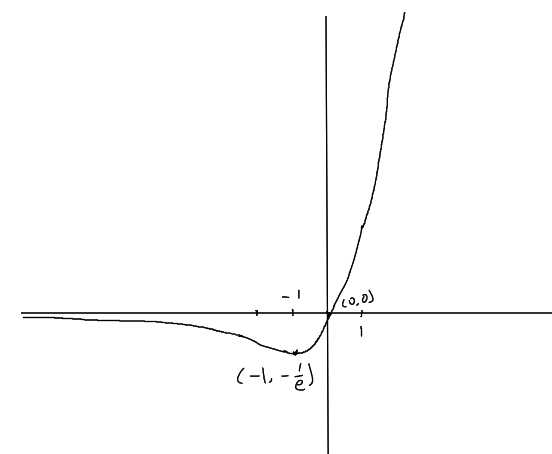
\includegraphics[width=0.6\linewidth]{q4.png}
\end{center}

\problem{5}
\begin{multicols}{2}
	\begin{itemize}
		\item[(b)]
		\begin{minipage}[t]{\linewidth}
			\begin{mdframed}
				\begin{align*}
					\Limit{1}{x^9-1}&=0 \\
					\Limit{1}{x^5-1}&=0
				\end{align*}
			\end{mdframed}
			\begin{align*}
				&\limit{1}\frac{x^9-1}{x^5-1}
				\lheqzero\limit{0}\frac{9x^8}{5x^4}
				=\limit{1}\frac{9x^4}{5}
				=\boxed{\frac95}
			\end{align*}
		\end{minipage}

		\item[(d)]
		\begin{minipage}[t]{\linewidth}
			\begin{mdframed}
				\begin{align*}
					\Limit[t]{0}{e^t-1}&=0 \\
					\limit[t]{0}t^3&=0
				\end{align*}
			\end{mdframed}
			\begin{equation*}
				\limit[t]{0}\frac{e^t-1}{t^3}
				\lheqzero\limit[t]{0}\frac{e^t}{t^2}
				=\boxed{\infty}
			\end{equation*}
		\end{minipage}

		\item[(e)]
		\begin{equation*}
			\limit{0}\frac{\cancel{\tan}(px)}{\cancel{\tan}(qx)}
			=\limit{0}\frac{p\cancel{x}}{q\cancel{x}}
			=\boxed{\frac pq}
		\end{equation*}

		\item[(f)]
		\begin{minipage}[t]{\linewidth}
			\begin{mdframed}
				\begin{align*}
					\limit{\infty}\ln x&=\infty \\
					\limit{\infty}\sqrt{x}&=\infty
				\end{align*}
			\end{mdframed}
			\begin{align*}
				&\limit{\infty}\frac{\ln x}{\sqrt{x}}
				\lheqinfty\limit{1}\frac{\frac{1}{x}}{\frac{1}{2\sqrt{x}}}
				=2\limit{\infty}\frac{\sqrt{x}}{x} \\
				={}&2\limit{\infty}\frac{\sqrt{x}}{\sqrt{x}\cdot\sqrt{x}}
				=2\limit{\infty}\frac{1}{\sqrt{x}}
				=\boxed{0}
			\end{align*}
		\end{minipage}

		\item[(j)]
		\begin{minipage}[t]{\linewidth}
			\begin{mdframed}
				\begin{align*}
					\Limit[t]{0}{5^t-3^t}&=1-1=0 \\
					\limit[t]{0}t&=0
				\end{align*}
			\end{mdframed}
			\begin{align*}
				&\limit[t]{0}\frac{5^t-3^t}{t}
				\lheqzero\limit[t]{0}\frac{5^t\ln5-3^t\ln3}{1}
				=\boxed{\ln5-\ln3}
			\end{align*}
		\end{minipage}

		\item[(l)]
		\begin{minipage}[t]{\linewidth}
			\begin{mdframed}
				\begin{align*}
					\Limit{0}{1-\cos x}&=0 \\
					\limit{0}x^2&=0
				\end{align*}
			\end{mdframed}
			\begin{align*}
				&\limit{0}\frac{1-\cos x}{x^2}
				\lheqzero\limit{0}\frac{\sin x}{2x}
				=\frac{1}{2}\limit{0}\frac{\sin x}{x}
				=\boxed{\frac12}
			\end{align*}
		\end{minipage}

		\item[(n)]
		\begin{minipage}[t]{\linewidth}
			\begin{mdframed}
				\begin{align*}
					\Limit{1}{1-x+\ln x}&=0 \\
					\Limit{1}{1+\cos\pi x}&=0
					\Limit{1}{-1+\frac1x}&=0 \\
					\Limit{1}{-\pi\sin\pi x}&=0
				\end{align*}
			\end{mdframed}
			\begin{align*}
				&\limit{1}\frac{1-x+\ln x}{1+\cos\pi x}
				\lheqzero\limit{1}\frac{-1+\frac1x}{-\pi\sin\pi x} \\
				\lheqzero{}&\limit{1}\frac{-\frac{1}{x^2}}{-\pi^2\cos\pi x}
				=\frac{-1}{-\pi^2\cos\pi}
				=\boxed{-\frac{1}{\pi^2}}
			\end{align*}
		\end{minipage}

		\item[(p)]
		\begin{minipage}[t]{\linewidth}
			Let $y=1/x$. Then $x=1/y$ and $\pi/x=\pi y$. As $x\to\infty$, $y\to0$.
			\begin{align*}
				&\limit{\infty}x\sin\frac{\pi}{x}
				=\limit[y]{0}\frac{1}{y}\sin\pi y
				=\limit[y]{0}\frac{\sin\pi y}{y} \\
				\shortintertext{
					\begin{mdframed}
						\begin{align*}
							\limit[y]{0}\sin\pi y&=0 \\
							\limit[y]{0}y=0
						\end{align*}
					\end{mdframed}
				}
				\lheqzero{}&\limit[y]{0}\frac{\pi\cos\pi y}{1}
				=\boxed{\pi}
			\end{align*}
		\end{minipage}

		\item[(r)]
		\begin{minipage}[t]{\linewidth}
			\begin{align*}
				&\limit{\infty}x^3e^{-x^2}
				=\limit{\infty}\frac{x^3}{e^{x^2}}
				\shortintertext{
					\begin{mdframed}
						\begin{align*}
							\limit{\infty}x^3&=\infty \\
							\limit{\infty}e^{x^2}&=\infty \\
							\limit{\infty}3x&=\infty \\
							\limit{\infty}2e^{x^2}&=\infty
						\end{align*}
					\end{mdframed}
				}
				\lheqinfty{}&\limit{\infty}\frac{3x^{\cancel{2}}}{2\cancel{x}e^{x^2}}
				\lheqinfty\limit{\infty}\frac{3}{2\cdot2x\cdot e^{x^2}}
				=\boxed{0}
			\end{align*}
		\end{minipage}

		\item[(s)]
		\begin{minipage}[t]{\linewidth}
			\begin{align*}
				&\limit{1^+}\ln x\tan\frac{\pi x}{2}
				=\limit{1^+}\frac{\ln x\sin\frac{\pi x}{2}}{\cos\frac{\pi x}{2}}
				\shortintertext{
					\begin{mdframed}
						\begin{align*}
							\limit{1^+}\ln x\sin\frac{\pi x}{2}&=0 \\
							\limit{1^+}\cos\frac{\pi x}{2}&=0
						\end{align*}
					\end{mdframed}
				}
				\lheqzero{}&\limit{1^+}\frac{\frac{\sin\frac{\pi x}{2}}{x}-\ln(x)\cdot\frac{\pi}{2}\cdot\cos\frac{\pi x}{2}}{-\frac{\pi}{2}\sin\frac{\pi x}{2}} \\
				={}&\frac{\frac{1}{1}-0\cdot\frac{\pi}{2}\cdot0}{-\frac{\pi}{2}\cdot1}
				=\boxed{-\frac{2}{\pi}}
			\end{align*}
		\end{minipage}

		\item[(t)]
		\begin{minipage}[t]{\linewidth}
			\begin{align*}
				&\Limit{1}{\frac{x}{x-1}-\frac{1}{\ln x}}
				=\limit{1}\frac{x\ln x-x+1}{(x-1)\ln x}
				\shortintertext{
					\begin{mdframed}
						\begin{align*}
							\Limit{1}{x\ln x-x+1}&=0 \\
							\limit{1}(x-1)\ln x&=0 \\
							\limit{1}\ln x&=0 \\
							\Limit{1}{\ln x+\frac{x-1}{x}}&=0
						\end{align*}
					\end{mdframed}
				}
				\lheqzero{}&\limit{1}\frac{\ln x+x\cdot\frac1x-1}{\ln x+\frac{x-1}{x}}
				=\limit{1}\frac{\ln x}{\ln x+\frac{x-1}{x}} \\
				\lheqzero{}&\limit{1}\frac{\frac{1}{x}}{\frac{1}{x}+\frac{x-(x-1)}{x^2}}
				=\limit{1}\frac{1}{x\paren{\frac1x+\frac{1}{x^2}}} \\
				={}&\frac{1}{1(1+1)}=\boxed{\frac12}
			\end{align*}
		\end{minipage}

		\item[(u)]
		\begin{minipage}[t]{\linewidth}
			\begin{align*}
				&\Limit{\infty}{\sqrt{x^2+x}-x} \\
				={}&\Limit{\infty}{\sqrt{x^2}\sqrt{1+\frac1x}-x} \\
				={}&\Limit{\infty}{|x|\sqrt{1+\frac1x}-x} \\
				={}&\limit{\infty}x\paren{\sqrt{1+\frac1x}-1} \\
				\shortintertext{Let $y=1/x$. Then $x=1/y$. As $x\to\infty$, $y\to0$.}
				={}&\limit[y]{0}\frac1y\paren{\sqrt{1+y}-1}
				=\limit[y]{0}\frac{\sqrt{1+y}-1}{y}
				\shortintertext{
					\begin{mdframed}
						\begin{align*}
							\Limit[y]{0}{\sqrt{1+y}-1}&=0 \\
							\limit[y]{0}y&=0
						\end{align*}
					\end{mdframed}
				}
				\lheqzero{}&\limit[y]{0}\frac{\frac{1}{2\sqrt{1+y}}}{1}
				=\frac{1}{2\sqrt{1+0}}=\boxed{\frac12}
			\end{align*}
		\end{minipage}
	\end{itemize}
\end{multicols}

\end{document}
